\chapter{Extracción de normales mediante síntesis de alto nivel}

\section{Introducción}
Se ha expuesto en el capítulo anterior cómo es el proceso de obtención de vectores normales a una superficie definida por una nube de puntos. Además, se ha indicado qué parte de dicho proceso será objeto de aceleración con hardware digital: la obtención de matrices de covarianzas y el centroide a partir de un conjunto de puntos de la nube.
\\
\\
En el presente capítulo se exponen las diferencias entre el código original y el modificado para que sea sintetizable en hardware. Tras esto, se indicarán las optimizaciones realizadas sobre el código modificado y la generación de la IP (Intellectual Property) para el posterior trabajo con ella. Para ello se empleará Vivado HLS, una herramienta de síntesis de alto nivel para llevar a cabo la síntesis del algoritmo software en un IP hardware.


\section{Algoritmo original de estimación de matrices de covarianzas}

En la librería PCL se puede encontrar el método que permite calcular la matriz de covarianzas asociada a un punto estudiado y sus vecinos dentro de la nube de puntos original sobre la que se desean obtener los vectores normales\cite{calculo_covarianzas}. Sobre éste el autor del presente trabajo realiza las modificaciones pertinentes para que el código resultante sea sintetizable en hardware.
\\
\\
Como se ha explicado previamente, el método \textit{computeMeanAndCovarianceMatrix} recibe como argumentos la nube de puntos original como \textit{cloud}, un vector que contiene los índices de los puntos que forman una vecindad entorno al punto estudiado en la iteración actual llamado \textit{indices} así como \textit{covariance\_matrix} y \textit{centroid} para guardar respectivamente la matriz de covarianzas y el centroide obtenidos.

\begin{lstlisting}[language=C++,breaklines]
  template <typename PointT, typename Scalar> inline unsigned int
pcl::computeMeanAndCovarianceMatrix (const pcl::PointCloud<PointT> &cloud,
                                     const std::vector<int> &indices,
                                     Eigen::Matrix<Scalar, 3, 3> &covariance_matrix,
                                     Eigen::Matrix<Scalar, 4, 1> &centroid)
{
\end{lstlisting}

Aparece la librería Eigen para crear una matriz llamada \textit{accu} en la que guardar resultados intermedios. Se comprueba si el atributo \textit{is\_dense} de la nube \textit{cloud} es \textit{true} o \textit{false} para llevar a cabo las mencionadas operaciones intermedias de diferentes maneras. En cualquiera de los casos, se recorre todo el vector de índices para obtener los resultados adecuados en \textit{accu} que posteriormente se divide entre el número de elementos del vector \textit{indices}.


\begin{lstlisting}[language=C++,breaklines]

  Eigen::Matrix<Scalar, 1, 9, Eigen::RowMajor> accu = Eigen::Matrix<Scalar, 1, 9, Eigen::RowMajor>::Zero ();
  size_t point_count;
  if (cloud.is_dense)
  {
    point_count = indices.size ();
    for (size_t i = 0; i <= point_count; ++i)
    {
      accu [0] += cloud[indices[i]].x * cloud[indices[i]].x;
      accu [1] += cloud[indices[i]].x * cloud[indices[i]].y;
      accu [2] += cloud[indices[i]].x * cloud[indices[i]].z;
      accu [3] += cloud[indices[i]].y * cloud[indices[i]].y;
      accu [4] += cloud[indices[i]].y * cloud[indices[i]].z;
      accu [5] += cloud[indices[i]].z * cloud[indices[i]].z;
      accu [6] += cloud[indices[i]].x;
      accu [7] += cloud[indices[i]].y;
      accu [8] += cloud[indices[i]].z;
    }
  }
  else
  {
    point_count = 0;
    for (size_t i = 0; i <= indices.end(); ++i)
    {
      if (!isFinite (cloud[indices[i]]))
        continue;

      ++point_count;
      accu [0] += cloud[indices[i]].x * cloud[indices[i]].x;
      accu [1] += cloud[indices[i]].x * cloud[indices[i]].y;
      accu [2] += cloud[indices[i]].x * cloud[indices[i]].z;
      accu [3] += cloud[indices[i]].y * cloud[indices[i]].y;
      accu [4] += cloud[indices[i]].y * cloud[indices[i]].z;
      accu [5] += cloud[indices[i]].z * cloud[indices[i]].z;
      accu [6] += cloud[indices[i]].x;
      accu [7] += cloud[indices[i]].y;
      accu [8] += cloud[indices[i]].z;
    }
  }

  accu /= static_cast<Scalar> (point_count);
 \end{lstlisting}
 
Por último, se almacenan en \textit{centroid} y \textit{covariance\_matrix} los resultados finales del algoritmo.
 
 \begin{lstlisting}[language=C++,breaklines]
  centroid[0] = accu[6]; centroid[1] = accu[7]; centroid[2] = accu[8];
  centroid[3] = 1;
  covariance_matrix.coeffRef (0) = accu [0] - accu [6] * accu [6];
  covariance_matrix.coeffRef (1) = accu [1] - accu [6] * accu [7];
  covariance_matrix.coeffRef (2) = accu [2] - accu [6] * accu [8];
  covariance_matrix.coeffRef (4) = accu [3] - accu [7] * accu [7];
  covariance_matrix.coeffRef (5) = accu [4] - accu [7] * accu [8];
  covariance_matrix.coeffRef (8) = accu [5] - accu [8] * accu [8];
  covariance_matrix.coeffRef (3) = covariance_matrix.coeff (1);
  covariance_matrix.coeffRef (6) = covariance_matrix.coeff (2);
  covariance_matrix.coeffRef (7) = covariance_matrix.coeff (5);

  return (static_cast<unsigned int> (point_count));
}
\end{lstlisting}



\section{Algoritmo modificado e integración en Vivado HLS}
Se ha decidido seleccionar el cálculo de la matriz de covarianzas y centroide explicado en la figura \ref{fig:compute_computeMean} para su aceleración puesto que se reduce a operaciones con vectores y matrices que no requieren el uso de librerías específicas a diferencia del cálculo de las componentes del vector normal que necesita utilizar Eigen y complica la aceleración mediante hardware.
\\
\\
No solamente se mostrará a continuación el código modificado sino que se indicará su integración en el programa Vivado HLS, del cual se hace uso para la generación automática de hardware digital.
\\
\\
En primer lugar se crea un nuevo proyecto en Vivado HLS y se selecciona la placa de desarrollo con la que se trabaja en el presente trabajo, la PYNQ-Z1 con un SoPC xc7z020clg400-1.
\\
\\
A la hora de integrar en HLS el algoritmo de cálculo de matrices de covarianzas, se hace uso de tres archivos:

\begin{itemize}
\item[•] \textit{normal.cpp}: Es el código de PCL modificado que permite extraer matrices de covarianzas, además de ciertos aspectos añadidos pertenecientes a la síntesis hardware.
\item[•] \textit{normal\_tb.cpp}: Se trata de un test bench que comprueba el correcto funcionamiento de normal.cpp pues compara resultados reales con los simulados. Cabe destacar aquí que se ha modificado ligeramente la librería PCL para que tras cada cómputo de una matriz de covarianzas y centroide, éstos se guarden en un fichero de texto cada uno para así tener acceso a estos resultados en cualquier momento.
\item[•] \textit{normal.hpp}: Es el conjunto de herramientas y librerías necesarias para normal.cpp y normal\_tb.cpp
\end{itemize}

\subsubsection{normal.cpp}\label{explicacion_software}
Antes de escribir código en Vivado HLS para sintetizarlo en hardware se deben tener en cuenta las limitaciones del hardware respecto al software, es decir, ciertas prácticas software que no pueden sintetizarse en hardware o que dan problemas y por lo tanto hay que tomar diferentes aproximaciones para llevar a cabo el algoritmo deseado. 
\\
\\
Por lo tanto, deben realizarse modificaciones sobre el método \textit{computeMeanAndCovarianceMatrix} de forma que el código original quede mínimamnete alterado así como lo más cerca posible de la realidad hardware para que esta metodología o método de modificación sea extensible al resto de bloques de sistema de visión:

\begin{itemize}
\item[•] Trabajar con matrices en software es sencillo ya que una matriz de números enteros, por ejemplo, se trata de un conjunto de vectores de la misma dimensión y que conforman las filas de la matriz. Para trabajar con ella se tiene un puntero que apunta a $n$ punteros a entero, siendo $n$ el número de filas. En hardware es más sencillo trabajar directamente con arreglos o arrays, es decir, solamente vectores o punteros a entero y no un puntero que apunta a otro puntero. Por lo tanto, la matriz de covarianzas de dimensión 3x3 se trata como un vector de nueve elementos y la nube de puntos con la que se trabaja se divide en tres vectores: si la nube de puntos en forma matricial tiene $n$ filas (número de puntos) y tres columnas (coordenadas x, y, z de cada punto) ahora se tienen las tres columnas como tres vectores independientes que se llamarán \textit{cloud\_x}, \textit{cloud\_y} y \textit{cloud\_z}.

\item[•] Puesto que en la síntesis de hardware digital no se pueden tener variables de tamaño no fijo, es decir, no se pueden manejar herramientas de asignación dinámica de memoria, los argumentos \textit{cloud\_x}, \textit{cloud\_y}, \textit{cloud\_z} e \textit{indices} tienen un tamaño máximo del cual se utiliza el necesario según las variables \textit{num\_points} y \textit{num\_indices} que se refieren a las dimensiones de la nube y vector de índices respectivamente.

\item[•] todas las líneas que comienzan por ``\#pragma'' indican la creación de buses en los que agrupar variables para su interpretación en hardware. En concreto, el bus A contiene las entradas del algoritmo y el bus B las salidas. 

\item[•] Se ha eliminado la comprobación del atributo \textit{is\_dense} de la nube de puntos de entrada puesto que se no trabaja con nubes que contienen puntos cuya posición no esté determinada por un valor finito.

\item[•] Todas las instancias pertenecientes a la clase Eigen han sido suprimidas y sustituidas por variables del tipo correspondiente como es en el caso de la variable \textit{covariance\_matrix} que es una matriz de tipo flotante.
\\
\\
El código modificado queda entonces de la siguiente forma:
\end{itemize}

 \begin{lstlisting}[language=C++,breaklines]
 #include "normal_fix.h"

int compute ( float covariance_matrix[9], float centroid[4], float cloud_x[MAXPOINTS], float cloud_y[MAXPOINTS], float cloud_z[MAXPOINTS],int indices[MAXINDICES], int num_points, int num_indices)
{

	//entradas
	#pragma HLS INTERFACE s_axilite port=cloud_x  bundle=BUS_A
	#pragma HLS INTERFACE s_axilite port=cloud_y  bundle=BUS_A
	#pragma HLS INTERFACE s_axilite port=cloud_z  bundle=BUS_A
	#pragma HLS INTERFACE s_axilite port=indices bundle=BUS_A
	#pragma HLS INTERFACE s_axilite port=num_indices bundle=BUS_A
	#pragma HLS INTERFACE s_axilite port=num_points bundle=BUS_A

	//salidas
	#pragma HLS INTERFACE s_axilite port=covariance_matrix  bundle=BUS_B
	#pragma HLS INTERFACE s_axilite port=centroid bundle=BUS_B
	#pragma HLS INTERFACE s_axilite port=num_points bundle=BUS_B

	//return
	#pragma HLS INTERFACE s_axilite port=return bundle=BUS_B


	float accu[9]={0};

	indices_loop:for(int i = 0;i<num_indices;i++){
		accu[0] += cloud_x[indices[i]] * cloud_x[indices[i]];
		accu[1] += cloud_x[indices[i]] * cloud_y[indices[i]];
		accu[2] += cloud_x[indices[i]] * cloud_z[indices[i]];
		accu[3] += cloud_y[indices[i]] * cloud_y[indices[i]];
		accu[4] += cloud_y[indices[i]] * cloud_z[indices[i]];
		accu[5] += cloud_z[indices[i]] * cloud_z[indices[i]];
		accu[6] += cloud_x[indices[i]];
		accu[7] += cloud_y[indices[i]];
		accu[8] += cloud_z[indices[i]];
	}

	for(int i = 0;i<9;i++){
		accu[i]/=num_indices;
	}
	centroid[0] = accu[6];
	centroid[1] = accu[7];
	centroid[2] = accu[8];
	centroid[3] = 1;

	covariance_matrix[0] = accu [0] - accu [6] * accu [6];
	covariance_matrix[1] = accu [1] - accu [6] * accu [7];
	covariance_matrix[2] = accu [2] - accu [6] * accu [8];
	covariance_matrix[4] = accu [3] - accu [7] * accu [7];
	covariance_matrix[5] = accu [4] - accu [7] * accu [8];
	covariance_matrix[8] = accu [5] - accu [8] * accu [8];

	covariance_matrix[3] = accu [1] - accu [6] * accu [7];
	covariance_matrix[6] = accu [2] - accu [6] * accu [8];
	covariance_matrix[7] = accu [4] - accu [7] * accu [8];


	return num_points;
}
}
\end{lstlisting}

Pero no basta con adaptar el código para que sea sintetizable en hardware digital, si se quiere obtener una aceleración del algoritmo se han de usar directivas: optimizaciones o variantes a la hora de realizar una misma operación de modo que lleve menos tiempo completarla. Para el caso, se utiliza la directiva de ``pipeline'' en el siguiente bucle que permite realizar tareas en paralelo en lugar de forma secuencial y por lo tanto reducir el tiempo total de ejecución del bucle siempre y cuando no haya dependencia entre resultados intermedios, esto es, si para obtener un resultado A es necesario conocer otro resultado B de antemano, su cálculo no puede realizarse en paralelo. En el bucle en el que se calculan las componentes de $accu$, estas operaciones pueden realizarse en paralelo porque no hay dependencia entre las mencionadas componentes.

 \begin{lstlisting}[language=C++,breaklines]
indices_loop:for(int i = 0;i<num_indices;i++){
		accu[0] += cloud_x[indices[i]] * cloud_x[indices[i]];
		accu[1] += cloud_x[indices[i]] * cloud_y[indices[i]];
		accu[2] += cloud_x[indices[i]] * cloud_z[indices[i]];
		accu[3] += cloud_y[indices[i]] * cloud_y[indices[i]];
		accu[4] += cloud_y[indices[i]] * cloud_z[indices[i]];
		accu[5] += cloud_z[indices[i]] * cloud_z[indices[i]];
		accu[6] += cloud_x[indices[i]];
		accu[7] += cloud_y[indices[i]];
		accu[8] += cloud_z[indices[i]];
	}
\end{lstlisting}

\subsubsection{normal\_tb.cpp}
Las operaciones realizadas por el test bench se resumen en los siguientes puntos:

\begin{itemize}
\item Creación de variables tales como tres vectores de tipo float que almacenan las coordenadas de todos los puntos de la nube (\textit{cloud\_x}, \textit{cloud\_y} y \textit{cloud\_z}), el vector de nueve elementos que almacena la matriz de covarianzas (\textit{covariance\_matrix}), vector de enteros que almacena los índices de los puntos de la nube que forman una vecindad (\textit{indices}), vector de tipo float que almacena las coordenadas del centroide del conjunto de puntos que forman una vecindad (\textit{centroid}) y las ya mencionadas \textit{num\_points} y \textit{num\_indices} como valores enteros.

\item La nube de puntos está almacenada en un fichero de formato .txt por lo que se efectúa su lectura y se almacena en \textit{cloud}. Se hace lo mismo con un fichero de texto que contiene los índices de los puntos que forman una vecindad: se leen de un fichero de texto y se almacenan en \textit{indices}.

\item Se llama al método implementado en \textit{normal.cpp} para obtener los resultados deseados en las variables \textit{covariance\_matrix} y \textit{centroid}

\item Se leen los ficheros de texto que contienen la matriz de covarianzas y el centroide calculados por el código original gracias a la modificación de la librería PCL previamente mencionada y se compara con los resultados obtenidos por el código modificado.
\end{itemize}

De aquí en adelante, se utilizará como referencia la nube de puntos bunny.pcd de la figura \ref{fig:bunny_ejemplo} y el conjunto de puntos representados por los siguientes índices para calcular su respectiva matriz de covarianzas y centroide:


\begin{lstlisting}[language=C++,breaklines]
int indices_sw[11]={396 ,382 ,392 ,381 ,389 ,395 ,391, 386 ,393, 394, 385 };
\end{lstlisting}

Estos son los índices correspondientes a la última iteración en el cálculo de matrices de covarianzas y se puede acceder a ellos tras la ejecución software del algoritmo gracias a las modificaciones realizadas por el autor en la librería PCL para poder almacenar en ficheros de texto la matriz de covarianzas y el centroide así como la nube de puntos con la que se trabaja y los diferentes conjuntos de índices de la misma que indican el los puntos con los que se opera en el algoritmo.
\\
\\
Se muestra en la imagen \ref{fig:resultados_hls} que el valor de la matriz de covarianzas y el centroide calculados con el código original de PCL y el modificado en Vivado HLS efectivamente coinciden. Esto se consigue con la herramienta de simulación del código, es decir, se corre el test bench que utiliza el algoritmo desarrollado en \textit{normal.cpp}

\begin{figure}[!htb]
\centering
\includegraphics[scale=0.7]{resultados_hls}
\caption{comparación de matriz de covarianzas y centroide obtenidos con Vivado HLS y PCL.}\label{fig:resultados_hls}
\end{figure}

\subsubsection{normal.hpp}
Se incluyen las librerías necesarias y se declaran las variables y el método que se usan en normal\_tb.cpp y normal.cpp además de definir las constantes ``MAXPOINTS'' y ``MAXINDICES'' que son las dimensiones máximas de la nube de puntos y el vector de índices como ya se ha discutido previamente sobre la imposibilidad de utilizar memoria dinámica en hardware.

\begin{lstlisting}[language=C++,breaklines]
#include <stdio.h>
#include <iostream>
#include <math.h>
#include <fstream>
#include <stdlib.h>
#include <vector>


#define MAXPOINTS 15000
#define MAXINDICES 20



int compute(  float covariance_matrix[9],
		  float centroid[4],
		  float cloud_x[MAXPOINTS],
		  float cloud_y[MAXPOINTS],
		  float cloud_z[MAXPOINTS],
		  int indices[MAXINDICES],
		 int num_points,
		 int num_indices);

\end{lstlisting}


\subsection{Generación de síntesis e IP}

Sabiendo que los resultados obtenidos con PCL y HLS coinciden, se procede a la ejecución de la síntesis para estimar el uso de los recursos hardware de los que dispone la FPGA. Así pues, en la figura \ref{fig:resultados_sintesis_hls} se puede ver un uso del 10\% de la memoria disponible así como un 11\% y 29\% de flip flops y lookup tables respectivamente. El recurso más variable es la memoria en forma de block RAM o BRAM ya que depende del tamaño de la nube con la que se trabaja y por tanto la cantidad de información que tiene que manejar la FPGA. En la figura \ref{fig:resultados_sintesis_hls2} se aprecian resultados referentes a tiempos y latencia en forma de ciclos de reloj necesarios para ejecutar el algoritmo.
\\
\\
\begin{figure}[!htb]
\minipage{0.48\textwidth}
  \includegraphics[width=\linewidth]{resultados_sintesis_hls}
  \caption{Estimación de utilización de recursos de la FPGA.}\label{fig:resultados_sintesis_hls}
\endminipage\hfill
\minipage{0.48\textwidth}
  \includegraphics[width=\linewidth]{resultados_sintesis_hls2}
  \caption{Estimación de latencia y tiempos en la FPGA.}\label{fig:resultados_sintesis_hls2}
\endminipage\hfill
\end{figure}

Tras comprobar que la FPGA tiene un uso correcto de sus recursos se puede exportar el Register Transfer Level (RTL) y generar la IP mediante la opción ``export RTL'' especificando que sea descrita en VHDL. Este bloque IP, que se llamará ``compute'', se utilizará en Vivado para configurar la FPGA para la aplicación del presente trabajo, acelerar el cálculo de la matriz de covarianzas.

\begin{figure}[!htb]
\centering
\includegraphics[scale=0.7]{export_RTL}
\caption{Exportación de RTL y generación de IP.}\label{fig:export_RTL}
\end{figure}

\section{Implementación de la IP en Vivado}
Teniendo exportada la IP que permite calcular matrices de covarianzas mediante hardware, se ha de configurar la FPGA con dicha funcionalidad.
\\
\\
Se crea un nuevo proyecto en el programa Vivado y se genera un diagrama de bloques como se muestra en la figura \ref{fig:diagrama_vivado} sobre el cual se destaca:
\begin{itemize}
\item[•] \textbf{processing\_system7\_0}: Se trata del Processing System (PS) explicado en el capítulo 2.
\item[•] \textbf{compute\_0}: Es la IP generada con Vivado HLS y que ha sido importada a Vivado.
\item[•] \textbf{system\_ila\_0}: Se trata del Integrated Logic Analyzer (ILA) y se encarga de tareas de debug haciendo uso de los propios recursos de la FPGA, puesto que los buses A y B contienen las entradas y salidas de \textbf{compute\_0} y las cuales se quieren controlar y observar.
\end{itemize}


\begin{figure}[!htb]
\centering
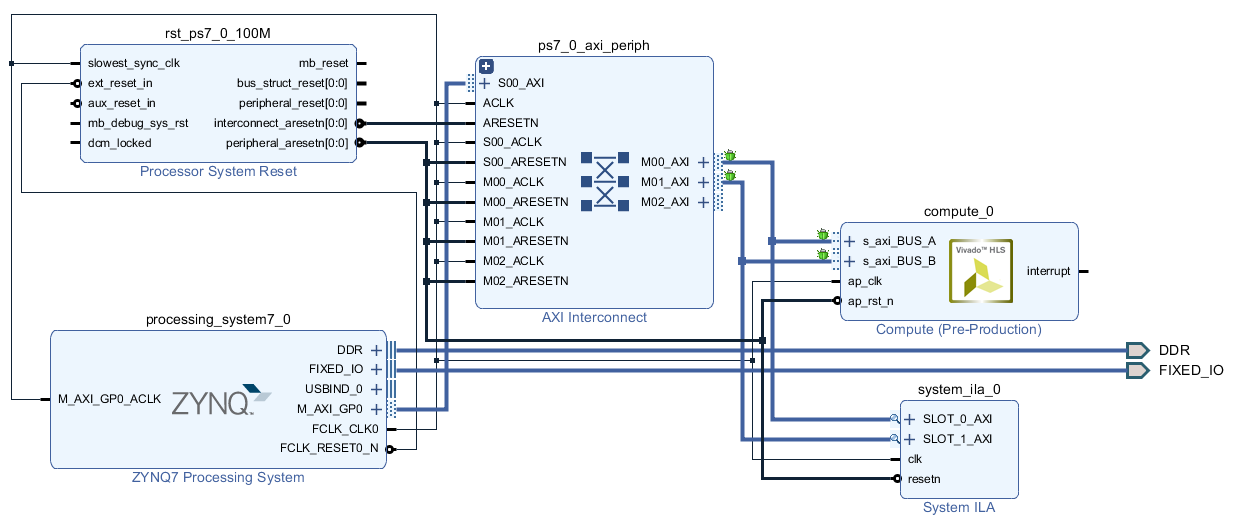
\includegraphics[scale=0.55]{diagrama_vivado}
\caption{Diagrama de bloques de la FPGA Pynq-Z1 y la IP de cálculo de matrices de covarianzas.}\label{fig:diagrama_vivado}
\end{figure}

Una vez comprobado que el diagrama es correcto se puede proceder a la generación del archivo de configuración que se cargará en la FPGA, el ``bitstream''. Esto se hace de forma automática y ofrece como resultado, a parte del mencionado archivo, una visión, en azul claro, de la distribución de los recursos utilizados en la capa de aplicación de la FPGA tal y como se aprecia en la figura \ref{fig:recursos_fpga}

\begin{figure}[!htb]
\centering
\includegraphics[scale=0.7]{recursos_fpga}
\caption{Recursos hardware utilizados para implementar la IP generada en Vivado HLS.}\label{fig:recursos_fpga}
\end{figure}

\section{Validacion del IP hardware sobre la FPGA}
El último paso antes de poder hacer uso de la IP ya configurada en la FPGA es comprobar que funciona adecuadamente sobre ésta. Para ello, utilizando Vivado, se exporta el hardware generado a un kit de desarrollo software (Software Development Kit o SDK) basado en Eclipse mediante el cual se puede hacer uso de la IP generada. El control de la IP en el entorno de desarrollo es posible porque junto al hardware se han exportado también unos drivers, una serie de funciones que permiten establecer las entradas del bloque IP, hacer que comience a calcular sus salidas y leerlas, entre otras operaciones.
\\
\\
En el SDK se abre un nuevo proyecto vacío basado en el hardware exportado desde Vivado, es decir, la configuración de la FPGA y que se encuentra en el entorno de trabajo del kit de desarrollo. Para utilizar la IP sobre la FPGA el autor ha creado un archivo en lenguaje C que sirve de test bench para comprobar el correcto funcionamiento del cálculo de matrices de covarianzas. Este archivo es muy similar al test bench ya creado y explicado en Vivado HLS pero tiene una diferencia: hay que comprobar que el cálculo de matrices de covarianzas da al mismo resultado ejecutándose mediante software (código en C compilado) y hardware (utilizando los drivers y los recursos hardware de la FPGA, es decir, su lógica programable PL) 
\\
\\
A efectos de cómo escribir el test bench afecta al desdoblamiento de variables, esto es, se necesitan dos variables que almacenen la matriz de covarianzas (y otros resultados finales y/o intermedios) en una de ellas la calculada mediante software y la otra mediante hardware.
\\
Además, la principal diferencia en este test bench comparado con el utilizado en Vivado HLS es el uso de la IP con sus respectivos drivers. Para ello, se crean las instancias de la IP de la siguiente manera:

\begin{lstlisting}[language=C++,breaklines]
	XCompute compute;
	XCompute_Config *compute_config = NULL;
\end{lstlisting}

$compute$ es la instancia de la IP, una estructura que contiene las direcciones de los buses A y B (entrada y salida) y $compute\_config$ una estructura que además de las mencionadas direcciones contiene el identificador de la IP. 
\\
\\
Para aportar los datos de entrada a la IP, se utilizan los siguientes métodos aportados por los drivers:

\begin{lstlisting}[language=C++,breaklines]
	XCompute_Write_covariance_matrix_Words(&compute, 0, covariance_matrix, 9);
	XCompute_Write_centroid_Words(&compute, 0, centroid, 4);

	XCompute_Write_indices_Words(&compute, 0, indices_sw, num_indices_hw);

	XCompute_Write_cloud_x_Words(&compute,0,cloud_x_sw,num_points_hw);
	XCompute_Write_cloud_y_Words(&compute,0,cloud_y_sw,num_points_hw);
	XCompute_Write_cloud_z_Words(&compute,0,cloud_z_sw,num_points_hw);
\end{lstlisting}

Donde $XCompute$ indica que el método se refiere a la IP $compute$ generada con Vivado HLS, $Write$ se refiere a que la operación es de escritura sobre la IP y el resto del nombre indica con qué señal se está operando, por ejemplo $indices\_words$ hace referencia al vector de índices de los puntos que conforman una vecindad. 
\\
Los parámetros que reciben estos métodos son, por orden, la instancia de la IP $compute$, la posición de memoria desde la que se quiere escribir el dato (0 para escribir el dato completo) la variable que almacena el dato que se desea escribir y por último la dimensión del mismo.
\\
\\
Con estos métodos se aporta a la IP una nube de puntos en forma de sus tres vectores de coordenadas, los índices de los puntos con los que estimar una matriz de covarianzas y centroide y las variables donde guardar resultados, es decir, centroide, matriz de covarianzas.
\\
\\
Para ejecutar el cálculo de la matriz de covarianzas con los datos aportados se llama al siguiente método:

\begin{lstlisting}[language=C++,breaklines]
	void compute_hw() {

	// Perform computation
	XCompute_Start(&compute);
	while (!XCompute_IsDone(&compute)) ; //Polling
}
\end{lstlisting}

Donde $XCompute\_Start(\&compute)$ inicia el cálculo de la matriz de covarianzas mediante hardware, indicando para ello la instancia a la IP deseada, en este caso, $compute$.
\\
\\
Por último, se llaman a métodos semejantes a los de escritura de datos sobre la IP pero en este caso sustituyendo en el nombre del método $Write$ por $Read$ por lo que queda de la forma:

\begin{lstlisting}[language=C++,breaklines]
	XCompute_Read_covariance_matrix_Words(&compute,0,covariance_matrix_hw, 9);
	XCompute_Read_centroid_Words(&compute,0,centroid_hw,4);

\end{lstlisting}

Con esto se consigue almacenar en la variable $covariance\_matrix\_hw$ la matriz de covarianzas y en $centroid\_hw$ el centroide.
\\
\\
Para el cálculo de la matriz de covarianzas y el centroide mediante software se procede de la forma explicada en el apartado \ref{explicacion_software} por lo que se crea un método para efectuar el mencionado cálculo.
\\
\\
Puesto que el objetivo es apreciar la aceleración del cálculo de la matriz de covarianzas y el centroide mediante hardware y respecto al software, se miden los tiempos de ejecución de cada tipo de cálculo.
\\
\\
Finalmente, tras cargar la nube $bunny.pcd$, que ya ha aparecido en el desarrollo de la memoria y puede verse de nuevo en la figura \ref{fig:bunny_ejemplo}, utilizando los correspondientes índices para calcular una de sus matrices de covarianzas y el centroide se obtienen los resultados de la figura \ref{fig:resultados_sdk} donde se puede apreciar que se obtiene una aceleración de más de un 160\% ($3.37\mu s$ con hardware y $5.58\mu s$ con software) así como se puede ver que los resultados obtenidos por software y hardware son idénticos y además coinciden con los de la simulación efectuada en Vivado HLS.
\\
\\
Queda demostrada entonces la aceleración que es posible conseguir sobre operaciones aritméticas tales como sumas, restas, multiplicaciones y divisiones que han de efectuarse cientos, miles o millones de veces sobre hardware en lugar de software.

\begin{figure}[!htb]
\centering
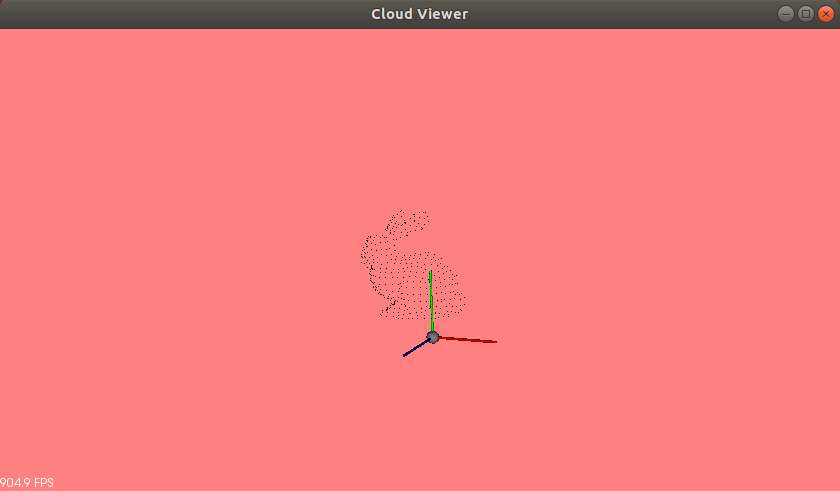
\includegraphics[scale=0.5]{bunny_ejemplo}
\caption{Nube de puntos bunny.pcd que representa un conejo con 397 puntos.}\label{fig:bunny_ejemplo}
\end{figure}


\begin{figure}[!htb]
\centering
\includegraphics[scale=0.8]{resultados_sdk}
\caption{Comparación de tiempos de cálculo de matriz de covarianzas y centroide entre software y hardware dada la nube bunny.pcd y 20 índices.}\label{fig:resultados_sdk}
\end{figure}




